\section{Theoretischer Hintergrund}
\label{th}
In dieser Sektion werden wichtige Grundlagen definiert und anhand von Beispielen erl\"autert. Zun\"achst folgt eine Einf\"uhrung in Artificial Neural Networks (zu Deutsch: \textit{Künstliche neuronale Netze}) in Sektion \ref{ann}. Daraufhin werden Convolutional Neural Networks (zu Deutsch etwa:\textit{Faltende neuronale Netze}) und ihre allgemeinen Bestandteile n\"aher erkl\"art (Sektion \ref{cnn}). 

\subsection{Artificial Neural Networks}
\label{ann}
Artificial Neural Networks (ANNs) sind im Machine Learning (zu Deutsch: \textit{Maschinelles Lernen}) angewandte Techniken, die von biologischen neuronalen Netzen inspiriert sind.  

Machine Learning ist ein Bereich der Informatik, in dem man Probleme durch Algorithmen l\"osen m\"ochte, welche keinen statisch programmierten L\"osungweg ben\"otigen. Das Ziel von Machine Learning ist das Konstruieren von Algorithmen, die anhand von Datens\"atzen Schlussfolgerungen ziehen k\"onnen und bei Eingabe unbekannter Daten diese Schlussfolgerungen zur Vorhersage von Ergebnissen generalisieren k\"onnen.

ANNs k\"onnen als gerichtete Graphen verstanden werden. Sie bestehen aus einer Menge an Knoten mit einer Menge an Kanten als Verbindungen zwischen den Knoten, welche die Aktivierungen der Knoten transportieren. Bei ANNs wird zwischen verschiedenen Strukturen unterschieden. In dieser Arbeit werden ausschlie\ss{}lich sogenannte feed-forward neural networks (zu deutsch etwa: \textit{vorw\"arts gekoppelte neuronale Netze}) genutzt. In feed-forward neural networks sind Knoten in Layern (zu Deutsch: \textit{Schichten}) angeordnet, welche untereinander kommunizieren. Die Knoten in einem Layer senden somit Signale an Knoten in anderen Layern, k\"onnen allerdings keine Signale an Knoten des selben Layers senden. Des weiteren zeichnen sich feed-forward neural networks dadurch aus, dass ein Knoten eine Aktivierung immer nur zu dem Layer weitersendet, welcher als sein Nachfolger definiert ist. Es werden keine Aktivierungen an die voranstehenden Layer zurückgesendet. 

Neuronen in ANNs haben einen Bias und jede Verbindung zu anderen Neuronen ist mit einem Gewicht belegt. Die Werte beider Eigenschaften sind variabel und werden im Verlauf des Lernprozesses immer wieder angepasst. Au\ss{}erdem verf\"ugt jedes Neuron über eine Aktivierungsfunktion, welche die Ausgabe des Neurons abhängig vom Eingabewert definiert.

%Artificial neurons are assigned with a bias and connections between neurons have a weight assigned to them. Additionally, neurons have an activation function. An activation function defines the output of a node dependent on the given input. The output function is a function, that takes the computed activation and returns the final output, that is send to the next neuron. Artificial neurons are typically organized in layers. Those layers can perform different kinds of transformations of their inputs (e.g. pooling layers, convolutional layers, etc. when looking at CNNs). 



Abbildung \ref{fig:basictop} zeigt eine einfache Topologie eines ANNs. Eine Eingabe wird vom Input Layer (zu Deutsch: \textit{Eingabeschicht}) in den Hidden Layer (zu Deutsch: \textit{Versteckte Schicht}) gegeben und von diesem in die letzte Schicht, welche als Output Layer (zu Deutsch: \textit{Ausgabeschicht}) funktioniert weitergereicht. 

\begin{figure}[ht]
\centering
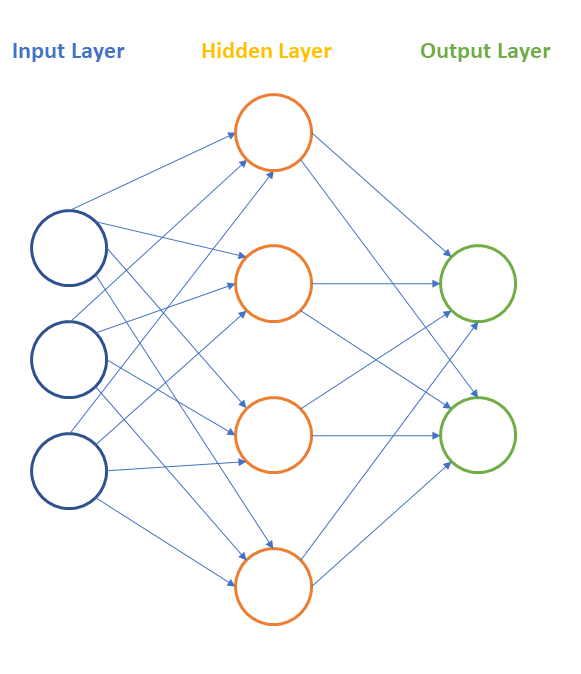
\includegraphics[scale=0.5]{pictures/grafiken/Folie3}
\caption[Caption for LOF]{Topologie eines einfachen ANNs.} 
\label{fig:basictop}
\end{figure}

Neural Networks (zu Deutsch: \textit{Neuronale Netze}) können als mathematische Modelle verstanden werden, welche eine Funktion $f : X \rightarrow Y$ definieren. In einem Neural Network wendet jedes Neuron eine Funktion auf seine Eingangswerte an, bevor es diese zur n\"achsten Schicht sendet. Somit kann die Funktion eines Neural Networks als eine Komposition aus jeder sich im Networks befindlichen Funktion definiert werden. 

Bezogen auf Abbildung \ref{fig:composedGraph}, sieht die zusammengesetzte Funktion des Networks wie folgt aus: 
\begin{equation}
\label{eq:compf}
f(g_1(h_1(x), h_2(x)),g_2(h_2(x), h_3(x)))
\end{equation}

\begin{figure}[ht]
\centering
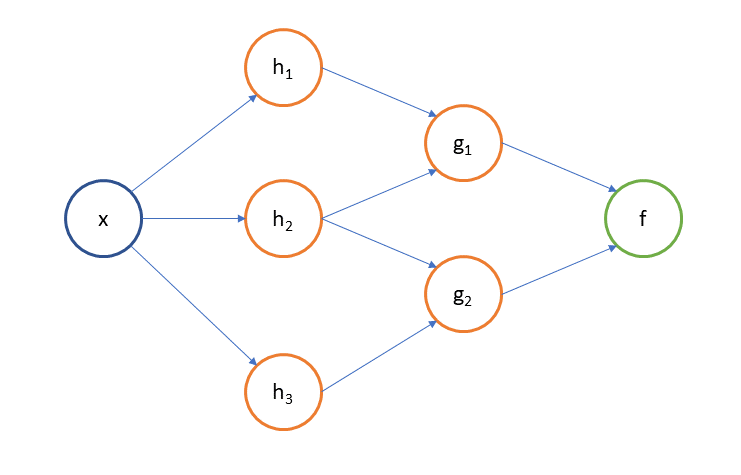
\includegraphics[scale=0.4]{pictures/grafiken/Folie4}
\caption[Caption for LOF]{Grafische Darstellung der zusammengesetzten Funktion $f$ aus Gleichung \ref{eq:compf}.}
\label{fig:composedGraph}

\end{figure}

\paragraph{Fully-connected layer}
Jeder Layer in einem klassischen ANN ist ein fully-connected Layer (zu Deutsch etwa: \textit{vollständig verbundene Schicht}). Neuronen in fully-connected Layern besitzen Verbindungen zu allen Neuronen des vorrangigen Layers. Jedes Neuron berechnet einen Ausgabewert $F(x)$ unter Verwendung des Eingabewertes \vect{x}, der Gewichte \mat{W}, die den Verbindungen zu dem vorherigen Layer zugewiesen sind, und eines Bias \vect{b}, der dem entsprechenden Neuron zugewiesen ist. 
\begin{equation}
\label{eq:fcl}
\begin{bmatrix}
w_{11} & ... & w_{1m}\\
. &  & .\\
. & . & .\\
. &  & .\\
w_{n1} & ... & w_{nm} 
\end{bmatrix} \cdot
\begin{bmatrix}
x_1\\
.\\
.\\
.\\
x_m
\end{bmatrix} + 
\begin{bmatrix}
b_1\\
.\\
.\\
b_n
\end{bmatrix} = 
\begin{bmatrix}
y_1\\
.\\
.\\
y_n
\end{bmatrix}
\end{equation}
Gleichung \ref{eq:fcl} zeigt die allgemeine Formel nach welcher der Ausgabewert eines fully-connected Layers berechnet wird. $n$ steht für die Anzahl der Neuronen im Layer und $m$ ist die Anzahl der Eingabewerte des vorherigen Layers. Die Gleichung kann auch wie folgt in Vektornotation formuliert werden: 
\begin{equation}
\label{eq:VecNot}
F(\vect{x}) = (\mat{W} \cdot \vect{x}) + \vect{b}^T
\end{equation} 
In Gleichung \ref{eq:VecNot} sind \mat{W} und \vect{b} lernbare Parameter, welche vom Optimierungsalgorithmus abgepasst werden k\"onnen. Sie stehen in der Gleichung f\"ur die Gewichte(\mat{W}) und den Bias(\vect{b}) des entsprechenden Layers.

\paragraph{Rectified Linear Units Layer}

In ANNs finden eine Vielzahl von Aktivierungsfunktionen Anwendung. Im Folgenden wir die ReLU-Funktion vorgestellt, da sie in den Modellen, die in dieser Arbeit implementiert werden genutzt wird. Sie ist wie folgt definiert: $relu(x) = max(0, x)$. Die Aktivierungsfunktion wird nach der Verarbeitung eingehender Werte im Neuron auf das Ergebnis angewandt und entfernt negative Werte aus dem Ausgabevektor des Neurons, bevor der Vektor an das n\"achste Layer weitergereicht wird \parencite{Wu.2017}.

\paragraph{Normalization Layer}

Das Normalization Layer (zu Deutsch: \textit{Normalisierungsschicht}) wird zur Normalisierung der Aktivierungen des vorherigen Layers genutzt. Nachfolgend wird ausschließlich batch normalization(BN) genutzt, da es sowohl f\"ur fully-connected Layer als auch f\"ur convolutional Layer genutzt werden kann und die Trainingsgeschwindigkeit des Netzwerks beschleunigt \parencite{DBLP:conf/icml/IoffeS15}.

\paragraph{Loss Function}

Die Loss Function (zu Deutsch: \textit{Verlustfunktion}) evaluiert wie genau ein Neural Network die ground-truth (zu Deutsch etwa: Grundwahrheit) der Trainingsdaten vorhersagt. Ihre Aufgabe besteht darin den Abstand zwischen der ground-truth \vect{(x, y)} einer Eingabe \vect{x} und der Vorhersage des ANNs $\hat{y}$. Neural Networks versuchen Gewichte und Biase so anzupassen, dass dieser Wert minimiert wird. Ein Beispiel f\"ur eine Loss function $z$ w\"are \parencite{Wu.2017}:

\begin{equation}
z = \frac{1}{2}\|\vect{(x, y)} - \hat{y}\|^2
\end{equation}


\paragraph{Softmax-Funktion}

Die Softmax-Funktion ist eine Variante der logisitschen Funktion. Die Funktion erh\"alt einen Vektor \vect{z} mit reellen Werten und einer beliebigen Dimension $K$ und verrechnet dessen Werte, so dass sich jeder Wert des Vektors \vect{z} im Bereich (0, 1] befindet und die Summe aller Werte 1 ergibt. Die Softmax-Funktion wird nach folgender Formel berechnet \parencite{Goodfellow-et-al-2016}:

\begin{equation}
softmax(\vect{z})_j = \frac{\mathrm{e}^{z_j}}{\sum_{k=1}^K \mathrm{e}^{z_k}}
\end{equation}
\\

Eine vollständige Funktion f\"ur das in Abbildung \ref{fig:basictop} gezeigte ANN w\"are:
\begin{multline*}
f(\mathbf{x}) = softmax(\mathbf{W_2} \cdot relu(\mathbf{W_1} \cdot \mathbf{x} + \mathbf{b_1}) + \mathbf{b_2} )
\end{multline*}


Der Eingabevektor \vect{x} ist in $\mathbb{R}^3$. Zuerst, wird \vect{x} vom Hidden Layer verarbeitet. In diesem Beispiel ist der Hidden Layer fully-connected, so dass die Formel f\"ur fully-connected Layer \ref{eq:fcl} mit $\mathbf{W_1}$ und $\mathbf{b_1}$ angewendet werden kann. $\mathbf{W_1}$ ist eine $4 \times 3$ Matrize und $\mathbf{b_1}$ ist in $\mathbb{R}^4$. Das Resultat wird mit einer Aktivierungsfunktion - in diesem Fall der ReLU-Funktion - verechnet und hat danach die Dimension $4\times1$. Daraufhin wird das Resultat an den Output Layer weitergegeben, welcher auch ein fully-connected Layer ist. Auch hier wird Gleichung \ref{eq:fcl} f\"ur fully-connected mit $\mathbf{W_2}$ als $2\times4$ Matrix und $\mathbf{b_2}$ als Vektor in $\mathbb{R}^2$ angewandt. Zuletzt wird die Softmax-Funktion auf das Ergebnis des Output Layers angewandt. Die Dimension des Ausgabevektors ist $2\times1$.


\subsection{Convolutional Neural Networks}

\label{cnn}

Ein Convolutional Neural Network (CNN) ist ein tiefes, feed-forward ANN. Es findet h\"aufig  Anwendung um Aufgaben im Zusammenhang mit Bildern, wie zum Beispiel Bildklassifikationen, zu l\"osen. Im Vergleich zu ANNs ben\"otigen CNNs im Allgemeinen weniger Gewichte, durch ihre Eigenschaft der lokalen Konnektivit\"at.

\"Ahnlich wie ANNs bestehen CNNs jeweils aus einem Input und einem Output Layer. Zwischen diesen beiden Layern befindet sich der Hidden Layer, in dem die Informationen aus den Eingabedaten haupts\"achlich verarbeitet werden. Der Hidden Layer kann aus verschiedenen Layer-Typen zusammengesetzt werden, welche beliebig untereinander kombiniert werden k\"onnen. Einige dieser Layer sind zum Beispiel: Convolutional, Pooling, fully-connected und Normalization Layer. In der Praxis sind ideale Layerzusammenstellungen stark an die Problemstellung gebunden und werden empirisch bestimmt. 

\paragraph{Convolutional layers}

Das Convolutional Layer ist einer der Kernbestandteile eines CNNs. Der Layer verf\"ugt \"uber einen Filter, bemessen durch einen Tensor des selben Ranges wie die Eingabedaten, welcher sogenannte Feature (zu Deutsch: \textit{Merkmale}) in den Eingabedaten detektiert. Filter sind durch ihre rezeptiven Felder charakterisiert, welche die Gr\"o\ss{}e der zeitgleich untersuchten Areale bestimmen \parencite{DBLP:journals/corr/OSheaN15}. Ein Beispiel f\"ur das rezeptive Feld eines Neurons k\"onnte eine $M \times N$ große Fl\"ache seine, welche kleinere oder gleich gro\ss{}e Abmessungen haben sollte wie die Dimensionen der Eingabedaten. Da die Tiefe des Filters $D_f$ \"aquivalent zu der Tiefe der Eingabedaten $D_i$ ist, ergibt sich $D_f = D_i$. Eingabewerte mit Dimensionen $10 \times 10 \times D_i$ w\"urde demnach in einem $M \times N \times D_i$ dimensionierten Filter mit $M, N \leq 10$ resultieren. 

Während der Filter die Eingabe verarbeitet, wird er \"uber die Eingabematrix geschoben und multipliziert die Werte in dem untersuchten Bereich mit den Werten seines Filters. Die Produkte werden zu einem einzigen Werte aufsummiert, welcher dann den Wert f\"ur das Areal widerspiegelt. Wenn der Prozess endet, ist das Ergebnis eine etwas kleinere Matrix, in welcher die aufsummierten Ergebnisse f\"ur jede m\"ogliche Position des Filters in den Eingabedaten erfasst sind. Aufbauend auf dem Beispiel im vorherigen Absatz ergibt sich eine Ausgabedimension von $6\times6$ bei einem $10\times10$ Eingabewert und einem $5\times5$ Filter. Im Allgemeinen resultiert eine Eingabe mit Bemessung $H^l \times W^l \times D^l$ und einem Filter der Gr\"o\ss{}e $H \times W \times D^l \times D$ in einer Ausgabe der Dimension $(H^l - H + 1) \times (W^l - W + 1) \times D$. In dieser Notation verweist $l$ auf den vorherigen Layer \parencite{Wu.2017}.

Sollte eine Ausgabe mit den selben Dimensionen wie die Eingabe ben\"otigt werden, so ist es m\"oglich \textit{padding} (zu Deutsch in etwa: \textit{Polsterung}) zu nutzen, um der Matrix Spalten und Zeilen nach Bedarf hinzuzuf\"ugen. Um die Dimensionen der Eingabematrix zu erhalten, m\"ussen $\lfloor \frac{H-1}{2} \rfloor$ Zeilen oberhalb der ersten Zeile und $\lfloor \frac{H}{2} \rfloor$ unterhalb der letzten Zeile hinzugef\"ugt werden. Außerdem m\"ussen $\lfloor \frac{W-1}{2} \rfloor$ Spalten vor der ersten Spalte und $\lfloor \frac{W}{2} \rfloor$ Spalten nach der letzten Spalte eingef\"ugt werden. Der Notation der vorangegangenen Abs\"atze folgend, beziehen sich $W$ und $H$ auf die vertikale und horizontale Dimension des Filters.

Zus\"atzlich kann ein \textit{stride}-Parameter (zu Deutsch: \textit{Schritt-Parameter}) $s$ definiert werden. Dieser Parameter bestimmt um wie viele Stellen der Filter nach jeder Rechnung auf der Matrix verschoben wird. Wenn jede m\"ogliche Position auf der Matrix evaluiert werden soll, betr\"agt der Wert des stride-Parameters $s=1$. F\"ur alle $s > 1$ wird der Filter $s - 1$ Positionen entlang beider Axen \"uberspringen.

Der Vorgang des "Abgehens" der Eingabewerte kann durch eine mathematische Formel [\ref{eq:convolution}] beschrieben werden. In der Formel ist der stride-Parameter $s=1$ und es findet kein padding statt. Die Notation folgt der bereits etablierten Notation und $H^{l+1}$, $W^{l+1}$ und $D^{l+1}$ beziehen sich auf H\"ohe, Breite und Tiefe der Ausgabematrix.
 
\begin{equation}
y \in \mathbb{R}^{H^{l+1} \times W^{l+1} \times D^{l+1}}
\end{equation}

mit $H^{l+1} = H^l - H + 1$, $W^{l+1} = W^l - W + 1$, and $D^{l+1} = D$ \parencite{Wu.2017}.


\begin{equation}
\label{eq:convolution}
y_{i',j',di} = \sum_{i=0}^{H}\sum_{j=0}^{W}\sum_{d =0}^{D^l} f_{i,j,d,di} \cdot x^{l}_{i'+i, j'+j, d}
\end{equation}

$f$ bezeichnet die Menge aller Filter und $x^l$ ist die Ausgabe des vorherigen Layers. Die Gleichung \ref{eq:convolution} wird \"uber die komplette Tiefe $D^l$ der Eingabe wiederholt ($0 \leq di \leq D^l$). Sie wird lediglich auf Positionen $(i',j')$ angewandt, welche die Bedingungen $0 \leq i' < H^{l + 1}$ und $0 \leq j' < W^{l + 1}$ erfüllen \parencite{Wu.2017}.

Im Bezug auf hoch dimensionierte Eingabewerte k\"onnen fully-connected neural networks r\"aumliche Abh\"angigkeiten nicht nutzen, da jedes Neuron vom jedem Neuron des vorherigen Layers Informationen sammelt und so immer alle Aktivierungen verarbeitet. Um r\"aumliche Informationen auszuwerten nutzen CNNs ein Pattern zur Erfassung lokaler Zusammenhänge. Aufgrund dieses Patterns, ist jedes Neuron nur mit einer kleinen Menge der Eingabegr\"o\ss{} verbunden. Hier wird nun das rezeptive Feld ben\"otigt, da es den Hyperparameter betitelt, welcher die r\"aumliche Bemessung des Sichtfeldes eines jeden Neurons abbildet.

\paragraph{Pooling layers}

Pooling Layer (zu Deutsch etwa: \textit{bündelnde Schicht}) werden auch als downsampling Layer bezeichnet. Ihre Aufgabe besteht darin die Ausgabewerte der vorherigen Layers in einen Wert zu kombinieren und somit die Dimensionen der weitergereichten Daten zu reduzieren. Abbildung \ref{fig:maxpool} zeigt eine bildliche Erkl\"arung des maxpool Layers.

\begin{figure}[H]
\centering
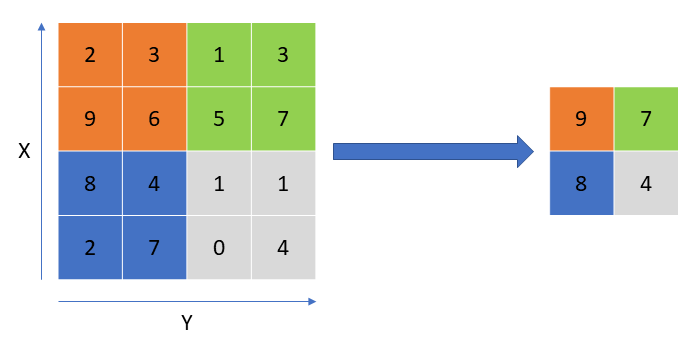
\includegraphics[scale=0.45]{pictures/grafiken/grafikenmax}
\caption[Caption for LOF]{Einfache Veranschaulichung des maxpool Layers mit $2 \times 2$ stride-Parameter.}
\label{fig:maxpool}

\end{figure}

Der maxpool Layer fu\ss{}t auf der Idee, dass die exakte Position eines Merkmals nicht so wichtig ist, wie seine Position in Relation zu anderen Merkmalen. Abh\"angig von der gestellten Aufgabe k\"onnte die Lage des Merkmals auch gar nicht relevant sein und die wichtige Information, die dieses Merkmal enth\"alt ist lediglich seine Existenz. Ein pooling Layer reduziert die Dimensionen der Eingabe in Abh\"angigkeit von seinen Parametern. So reduziert ein $2\times$ pooling Layer eine $8\times8$ dimensionierte Eingabe auf die Dimension $4\times4$, da es die Eingabematrix in sich nicht \"uberlappende $2\times2$ Quadrate unterteilt und f\"ur jedes Quadrat einen Wert errechnet, welcher in die Ausgabematrrix einflie\ss{}t. Die Inhalte der Ausgabe h\"angen von dem Typ des Layers ab, so errechnet ein maxpooling Layer immer die gr\"o\ss{}ten Werte beobachteten Bereichs, ein average-pooling Layer wiederum berechnet den Durchschnitt aller Werte in dem relevanten Bereich.

Der pooling Layer arbeitet auf der kompletten Tiefe der Eingabe und reduziert diese daher nicht, sondern berechnet jede Matrix unabh\"angig von den anderen. Die Eingabe wird somit lediglich in Breite und H\"ohe reduziert. Obwohl es auch andere Varianten der pooling Layer gibt, wie zum Beispiel average-pooling oder L2-norm pooling, wird haupts\"achlich maxpooling in den bekanntesten Architekturen verwendet.

Der Notation folgend resultiert ein pooling Layer der Gr\"o\ss{}e $(H \times W)$ in einer Ausgabe $H^{l+1} \times W^{l+1} \times D^{l+1}$. Unter der Annahme, dass $H$ und $W$, $H^l$ und $W^l$ teilen, gilt \parencite{Wu.2017}:

\begin{equation}
H^{l+1} = \frac{H^l}{H}, W^{l+1} = \frac{W^l}{W}, D^{l+1} = D^l.
\end{equation} 

Ein maxpooling Layer kann wie folgt definiert werden:

\begin{equation}
y_{i', j', d} = \max_{0 \leq i<H, 0 \leq j <W} x^{l}_{i' \cdot H + i, j' \times W + j, d}
\end{equation}

es gilt $0 \leq i' < H^{l+1}, 0 \leq j' < W^{l+1}$, und $0 \leq d < D^{l+1} = D^l$.  